\documentclass[11pt,letterpaper]{article}
\usepackage[T1]{fontenc}
\usepackage[utf8]{inputenc}
\usepackage[scaled=0.95]{helvet}
\renewcommand{\familydefault}{\sfdefault}
\usepackage[letterpaper,top=0.9in,bottom=0.95in,left=1in,right=1in]{geometry}
\usepackage{microtype}
\usepackage{enumitem}
\usepackage{titlesec}
\usepackage{fancyhdr}
\usepackage{xcolor}
\usepackage{booktabs}
\usepackage{array}
\usepackage{graphicx}
\usepackage{textcomp}
\usepackage[hidelinks]{hyperref}
\urlstyle{same}
\newcommand{\docversion}{2026-10-23-06-55-02} % set by build.py (America/Toronto)
\hypersetup{pdfsubject={version \docversion},pdftitle={The parish of St Monica's charity returns (T3010), 2008 onward: data, method and figures}}

\setlength{\parindent}{0pt}
\setlength{\parskip}{0.5em}
\linespread{1.03}
\sloppy
\titleformat{\section}{\normalfont\large\bfseries}{\thesection}{0.6em}{}[\vspace{1pt}\titlerule]
\titlespacing*{\section}{0pt}{1.1em}{0.4em}
\titleformat{\subsection}{\normalfont\bfseries}{\thesubsection}{0.6em}{}
\titlespacing*{\subsection}{0pt}{0.8em}{0.25em}
\pagestyle{fancy}
\fancyhf{}
\renewcommand{\headrulewidth}{0pt}
\fancyfoot[C]{\footnotesize\color{gray}St Monica's parish, T3010 returns -- data note -- page \thepage}
\fancyfoot[R]{\tiny\color{gray}v.\,\docversion}
\newcommand{\repourl}{https://github.com/OpenMobilityData/Terrebonne-open-sources}
\newcommand{\folder}{2024-st-monica-cra-t3010}

\begin{document}

{\LARGE\bfseries The parish of St Monica's charity returns (T3010), 2008 onward}\par\medskip
{\large Data, method and figures}\par\medskip
{\small A resident of Côte-des-Neiges--Notre-Dame-de-Grâce, from public records. Version \docversion. Repository: \href{\repourl}{\repourl}, folder \texttt{\folder}.}

\section{Purpose and scope}

The parish of St Monica (La fabrique de la paroisse de Sainte-Monique, 6405 rue de Terrebonne) is a registered charity. Like every registered charity in Canada it files a yearly information return, form T3010, with the Canada Revenue Agency (CRA), and the financial section of that return is public. The parish's building stands on rue de Terrebonne, on the stretch where a protected bike lane was built in 2024, and the parish's situation has been raised in the public debate on that lane. This note documents the parish's returns as the CRA released them, explains how the tables and charts in this folder are produced from them, and reads the charts in the terms of the return itself. It does not attribute any figure to any cause; the returns do not carry that information.

The data cover fiscal years ending December 31. Years 2008 to 2018 are on file from a data request answered by the CRA on December 6, 2024 (section~\ref{sec:prov}). Years 2019 to 2023 appear in the charts and the table from an interim source: the figures the author transcribed from the CRA's Charities Listings « quick view » in November--December 2024 into a spreadsheet; they are marked as such (hatched bars, an asterisk in the table) and are to be replaced by the CRA's yearly open-data files, fetched by the script described in section~\ref{sec:method}. The descriptive paragraphs of section~\ref{sec:figures} concern the years on CRA file, 2008 to 2018.

\section{The T3010 return}

Form T3010 has a financial section (Section~D for charities reporting on the short form, Schedule~6 for the others) whose entries are numbered. The numbers used here are the CRA's own line numbers; the labels are in \texttt{derived/line\_labels.csv} with a status column: \emph{checked} where the line's meaning is confirmed by the data on file (a total that sums, a text line that names its content, a figure that matches the parish's own published balance sheet), \emph{form} where the label is taken from the form and not independently confirmed, \emph{unverified} where the line's meaning has changed between form versions. The CRA publishes the form and its guide (T4033) on canada.ca, and a data dictionary with each open-data release.

The lines used in the figures are:
\begin{itemize}[nosep,leftmargin=1.4em]
\item \textbf{4700} total revenue; \textbf{4500} the total eligible amount of gifts for which the charity issued tax receipts; \textbf{4530} other gifts (no receipt); \textbf{4650} other revenue not already included, which line 4655 describes in 2011 as « Masses, funeral, weddings etc »; \textbf{4610} gross income from the rental of land or buildings; \textbf{4580} interest and investment income; \textbf{4540}, \textbf{4550}, \textbf{4560} revenue from the federal, provincial and municipal governments;
\item \textbf{5100} total expenditures; \textbf{4880} total compensation; \textbf{4850} occupancy costs; \textbf{4840} office supplies and expenses; \textbf{4860} professional and consulting fees; \textbf{4920} all other expenditures, which line 4930 describes in 2011 as « Contributions to diocese GST \& QST » and in 2012 as « GST \& QST »;
\item \textbf{4200} total assets; \textbf{4100} cash, bank accounts and short-term investments; \textbf{4140} long-term investments; \textbf{4155} land and buildings in Canada (on the 2008 form the same figure sits on line 4160); \textbf{4350} total liabilities.
\end{itemize}

\section{Provenance}\label{sec:prov}

\subsection{Years 2008 to 2018: the CRA's reply of December 6, 2024}

On November 10, 2024 the author asked the CRA's Charities Directorate, through the « Request publicly available data from the List of charities » web form, for the return data of the parish (business number 130341852RR0001) for the tax years 2008 to 2018 inclusive: general information, programs, the financial information (Section~D and Schedule~6), Schedule~5 and the directors' listing. The Directorate replied by e-mail on December 6, 2024 with four zip files of comma-separated values and this statement of the data's dates:

\begin{quote}\small
« You will also find the publicly available Basic contact information, General information, New and ongoing programs, Financial information, Non-cash gifts / gifts in kind (Schedule 5) and Directors, trustees, and like officials listings (Form T1235) data from the registered charity information return (T3010) for 2008 tax years as of September 7, 2017, the 2009 tax year as of June 30, 2018, the 2010 to 2012 tax years as of April 30, 2019, for the 2013 to 2016 tax years as of April 30, 2024 and for 2017 to 2018 tax year, as of October 31, 2024. »
\end{quote}

and this disclaimer:

\begin{quote}\small
« The information in this package contains data that the charitable organization sent to the Canada Revenue Agency (CRA). Please note that this data may have been manually entered by the CRA, and it has not necessarily been verified for accuracy or completeness by the CRA's Charities Directorate. »
\end{quote}

The files are kept unchanged in \path{raw/cra-charities-listings-2024-12-06/<year>/}, with the CRA's code lists in \texttt{references/} and the charity's listing record of October 31, 2024. Two kinds of file from the reply are not reproduced: the directors' listings (names of individuals) and the basic contact files (the 2008 one names the parish's contact person). The « as of » dates above are carried into every derived table as the \texttt{as\_of} column.

\subsection{Years 2019 and later: the CRA's open-data files}

Since 2019 the CRA has published the T3010 data of every registered charity on the Government of Canada's open-data portal, one dataset per fiscal year (« \textless year\textgreater\ List of charities », Open Government Licence -- Canada), as a set of CSV files: identification, general information, programs, the financial section, and others. Each file holds every charity. The script \texttt{derived/fetch\_open\_data.py} downloads the financial, general-information, identification and program files of a year, keeps the header and the parish's rows, and stores them in \path{raw/open-canada/<year>/} with the full file's URL, size and SHA-256 hash in \texttt{SOURCES.tsv}; the files about directors, trustees and like officials are never downloaded. These are extracts of a larger file and are labelled as such. The dataset identifiers known so far are in \texttt{derived/open\_canada\_datasets.csv}. The CRA's Charities Listings web application also shows each year's return (« quick view »). Figures typed from it go in \texttt{derived/manual\_entries.csv} with their source and the date they were viewed, and the build marks them as manual: the 2019--2023 values there are the author's transcription of November--December 2024. The build prefers a CRA file to a manual entry whenever both exist and reports every difference in \texttt{build\_report.txt}; the manual rows are to be removed once the files are in.

\section{Method}\label{sec:method}

\texttt{derived/build.py} does everything from the raw files:
\begin{enumerate}[nosep,leftmargin=1.6em]
\item reads every numbered field of the financial files (the 2008 reply is a single « T3010 Return » file; from 2009 the financial section is its own file) into one long table, \texttt{t3010\_lines.csv}: fiscal year, line, value, text (for the lines that carry a description), form identifier, source, « as of » date, file;
\item resolves one value per year and line, preferring the e-mailed CRA file, then the open-data extract, then a manual entry, and reports any disagreement between sources;
\item writes \texttt{t3010\_summary.csv}, one row per year with the lines listed in section~2, the land-and-buildings figure, and the difference between total revenue and total expenditures;
\item checks that line 4950 equals line 5100 and that the asset lines sum to line 4200, and writes what it found in \texttt{build\_report.txt};
\item draws the four charts in English and French (SVG and PNG) and writes the table of section~\ref{sec:figures} for this note, then stamps this note's version and compiles it.
\end{enumerate}

Charts: thin bars, a fixed order of colours checked for colour-vision deficiency with the validator of the chart-design method used across these repositories, a legend on every chart with more than one series, one axis per chart (thousands of dollars), the source line and the build date printed under each. In the stacked charts, « other lines » is the total line less the lines shown, so that each bar's height is the return's own total. The checks found one arithmetic gap in the data on file: in 2018 the four asset lines present sum to \$750,031 while line 4200 reads \$750,051.

\section{The figures}\label{sec:figures}

Table~\ref{tab:summary} gives the lines behind the charts, in dollars as filed; the years marked with an asterisk are from the interim transcription. All amounts are those of the returns; none is adjusted for prices. The paragraphs below describe the years on CRA file, 2008 to 2018.

\begin{table}[h]\centering\small
\caption{Key lines of the parish's T3010 returns (dollars as filed; * = interim transcription from the quick view, pending the CRA files; source and « as of » date per year in \texttt{t3010\_summary.csv}).}\label{tab:summary}
\resizebox{\textwidth}{!}{\begin{tabular}{@{}lrrrrrrrrrrrrrrrr@{}}\toprule
Line & 2008 & 2009 & 2010 & 2011 & 2012 & 2013 & 2014 & 2015 & 2016 & 2017 & 2018 & 2019* & 2020* & 2021* & 2022* & 2023* \\\midrule
4700 Total revenue & 291\,918 & 280\,506 & 305\,803 & 711\,793 & 383\,418 & 295\,774 & 412\,231 & 294\,600 & 304\,834 & 281\,819 & 296\,399 & 276\,981 & 211\,438 & 202\,900 & 259\,956 & 266\,650 \\
4500 Tax-receipted gifts & 233\,691 & 225\,815 & 266\,956 & 665\,140 & 336\,303 & 255\,609 & 373\,427 & 249\,079 & 252\,082 & 241\,808 & 254\,938 & 229\,425 & 195\,512 & 185\,599 & 190\,139 & 204\,950 \\
4530 Other gifts & -- & -- & -- & -- & -- & -- & -- & 24\,600 & 46\,244 & 36\,382 & 34\,787 & 34\,530 & 6\,602 & 9\,277 & 44\,861 & 29\,266 \\
4610 Rental income & 6\,621 & 5\,275 & 3\,700 & 5\,900 & 2\,500 & 5\,073 & 5\,335 & 7\,687 & 6\,141 & -- & 6\,435 & 8\,925 & 1\,175 & 3\,460 & 17\,490 & 15\,875 \\
4650 Other revenue & 44\,517 & 45\,642 & 63\,217 & 38\,840 & 42\,443 & 34\,943 & 32\,913 & 2\,387 & -- & 3\,365 & -- & -- & -- & -- & -- & 4\,943 \\
5100 Total expenditures & 305\,884 & 278\,268 & 301\,785 & 349\,750 & 871\,127 & 274\,310 & 326\,842 & 389\,129 & 297\,851 & 250\,879 & 261\,865 & 277\,716 & 198\,279 & 201\,549 & 291\,727 & 274\,890 \\
4880 Compensation & 123\,900 & 125\,990 & 124\,398 & 147\,183 & 137\,898 & 124\,299 & 124\,833 & 124\,576 & 130\,941 & 97\,314 & 114\,106 & 126\,787 & 72\,993 & 61\,370 & 116\,820 & 127\,217 \\
4850 Occupancy & 101\,670 & 74\,501 & 98\,270 & 108\,841 & 592\,737 & 76\,837 & 134\,024 & 164\,999 & 72\,746 & 50\,016 & 57\,730 & 57\,267 & 62\,123 & 58\,403 & 92\,477 & 49\,802 \\
4200 Total assets & 791\,096 & 813\,309 & 791\,356 & 1\,153\,027 & 663\,557 & 684\,600 & 766\,858 & 673\,901 & 680\,200 & 709\,620 & 750\,051 & 741\,843 & 794\,350 & 814\,638 & 723\,035 & 716\,315 \\
4100 Cash and short-term & 39\,857 & 44\,230 & 68\,574 & 231\,051 & 14\,765 & 73\,948 & 30\,391 & 36\,005 & 45\,242 & 71\,382 & 119\,181 & 108\,466 & 159\,474 & 139\,938 & 42\,378 & 31\,528 \\
4140 Long-term investments & 160\,000 & 160\,000 & 130\,000 & 330\,000 & 26\,124 & 26\,385 & 151\,941 & 52\,436 & 52\,804 & 53\,068 & 53\,307 & 53\,626 & 54\,326 & 100\,000 & 100\,600 & 105\,600 \\
4350 Total liabilities & 8\,737 & 28\,711 & 2\,747 & 2\,375 & 614 & -- & 239 & 1\,815 & 1\,128 & 489 & 8\,286 & 1\,414 & 40\,762 & 60\,000 & 268 & 2\,131 \\
Revenue less expenditures & -13\,966 & 2\,238 & 4\,018 & 362\,043 & -487\,709 & 21\,464 & 85\,389 & -94\,529 & 6\,983 & 30\,940 & 34\,534 & -735 & 13\,159 & 1\,351 & -31\,771 & -8\,240 \\\bottomrule
\end{tabular}
}
\end{table}

\subsection{Revenue and expenditures}

\begin{center}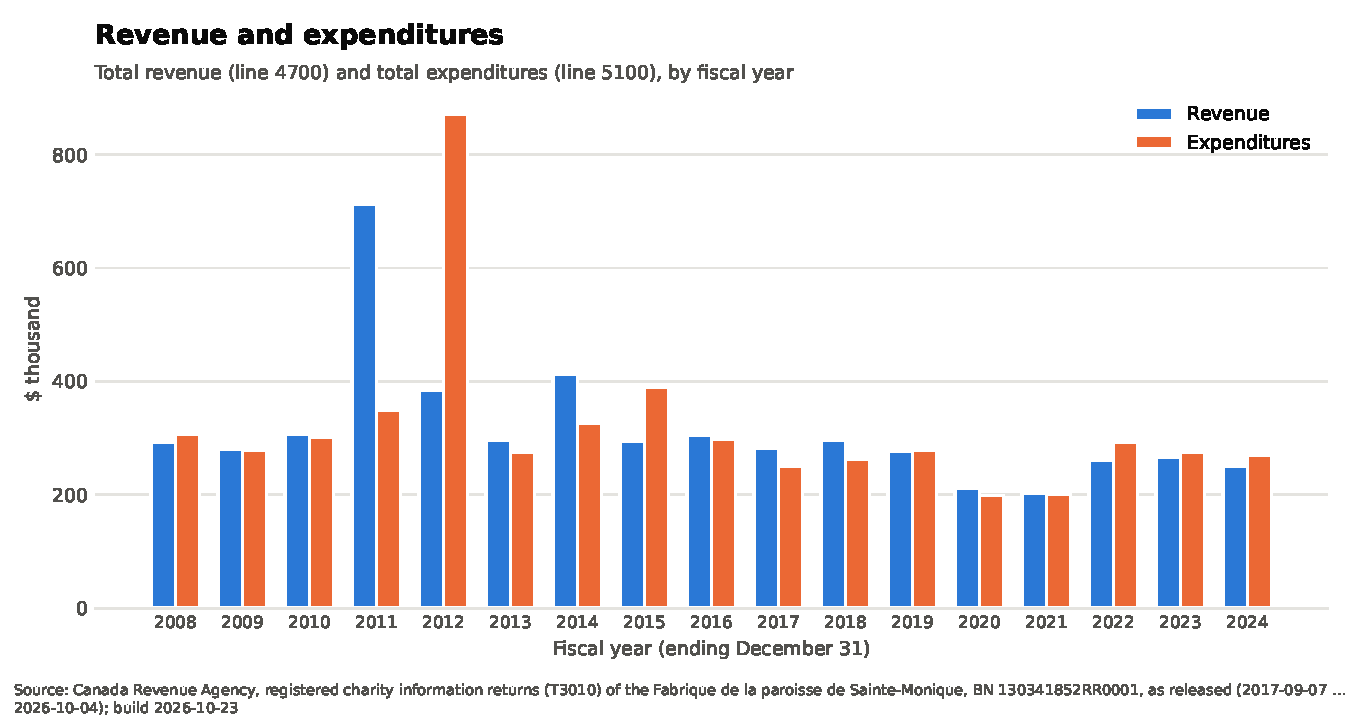
\includegraphics[width=\textwidth]{figures/revenue_and_expenditures_en.pdf}\end{center}

Total revenue (line 4700) lies between \$280,506 (2009) and \$305,803 (2010) in eight of the eleven years. The exceptions are 2011 (\$711,793), 2012 (\$383,418) and 2014 (\$412,231). Total expenditures (line 5100) lie between \$250,879 (2017) and \$305,884 (2008) in seven years; the exceptions are 2011 (\$349,750), 2012 (\$871,127), 2014 (\$326,842) and 2015 (\$389,129). Revenue exceeded expenditures in 2009, 2010, 2011, 2013, 2014, 2016, 2017 and 2018; expenditures exceeded revenue in 2008 (by \$13,966), 2012 (by \$487,709) and 2015 (by \$94,529).

\subsection{Revenue by line}

\begin{center}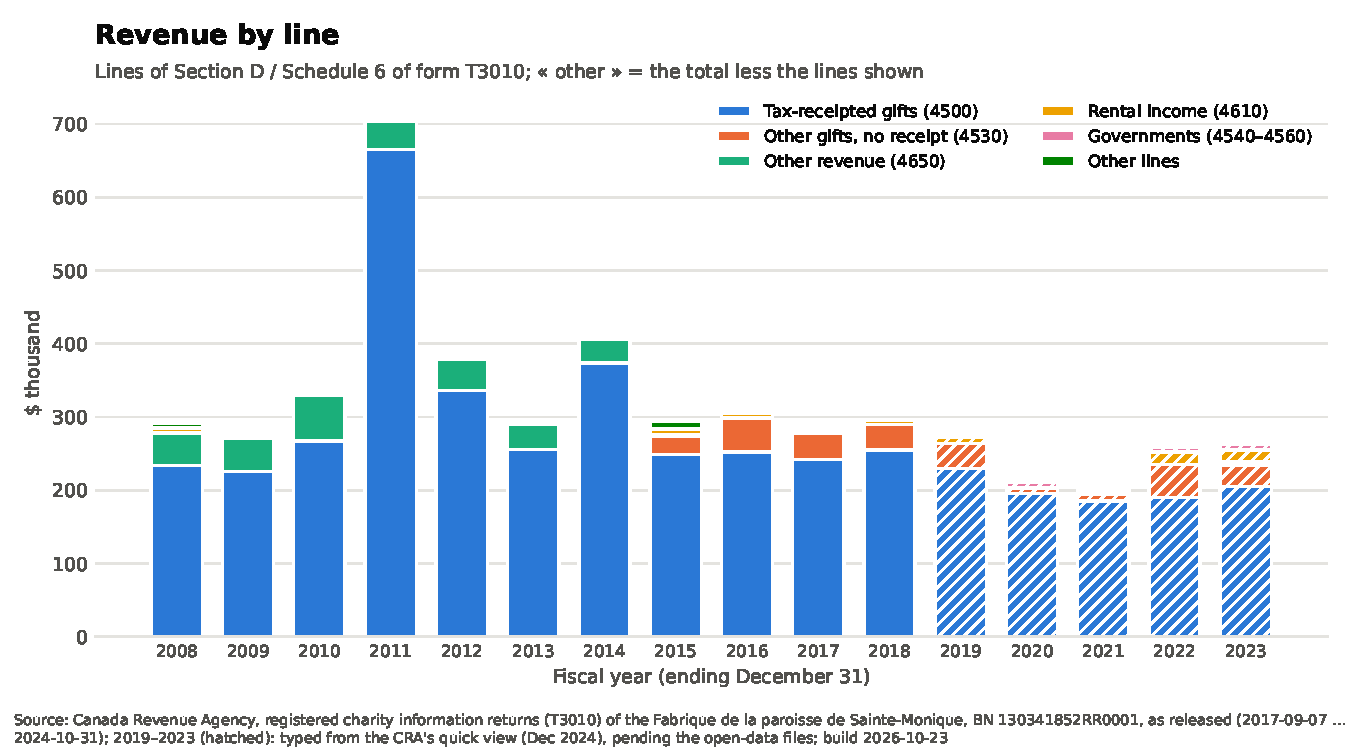
\includegraphics[width=\textwidth]{figures/revenue_by_line_en.pdf}\end{center}

Tax-receipted gifts (line 4500) are the largest line every year: \$225,815 to \$266,956 in 2008--2010 and 2013--2018 except 2014 (\$373,427), and \$665,140 in 2011. « Other revenue » (line 4650, described in 2011 as masses, funerals and weddings) is \$32,913 to \$63,217 from 2008 to 2014, then \$2,387 in 2015 and \$3,365 in 2017, and absent in 2016 and 2018; from 2015 a line that was empty before, other gifts without receipt (4530), carries \$24,600 to \$46,244. Rental income (4610) is \$2,500 to \$7,687 in the ten years where it is present (none in 2017); interest and investment income (4580) is \$6,707 in 2008 and \$45 to \$3,278 afterwards; no revenue from governments is reported in these years.

\subsection{Expenditures by line}

\begin{center}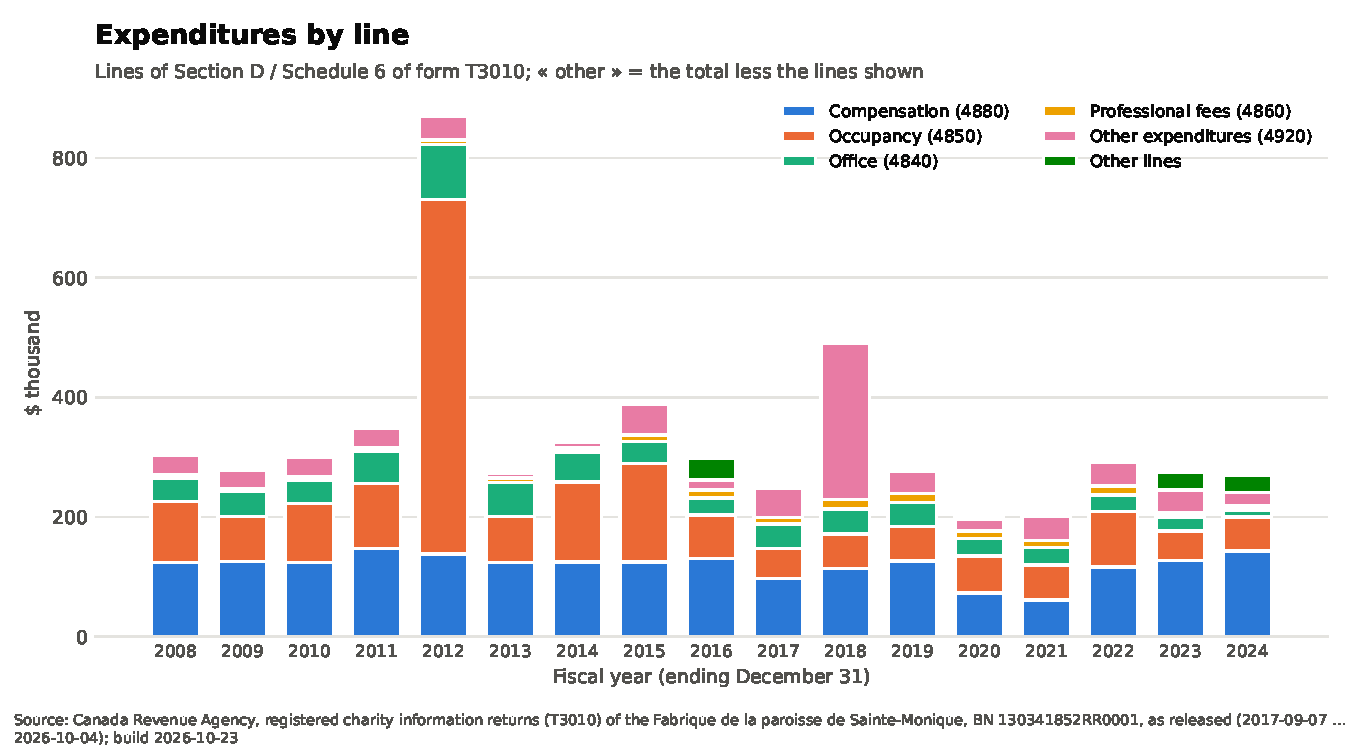
\includegraphics[width=\textwidth]{figures/expenditures_by_line_en.pdf}\end{center}

Compensation (line 4880) is the largest expenditure line in every year but 2012: \$97,314 (2017) to \$147,183 (2011). Occupancy costs (4850) are \$50,016 (2017) to \$164,999 (2015) in ten years and \$592,737 in 2012, the year of the largest total. Office expenses (4840) are \$28,196 to \$92,281; professional fees (4860) \$5,400 to \$15,428; the « all other » line (4920, described as contributions to the diocese and sales taxes) \$7,245 to \$50,844. The 2018 return carries no value on line 4950 and \$261,865 on line 5100.

\subsection{Assets by line}

\begin{center}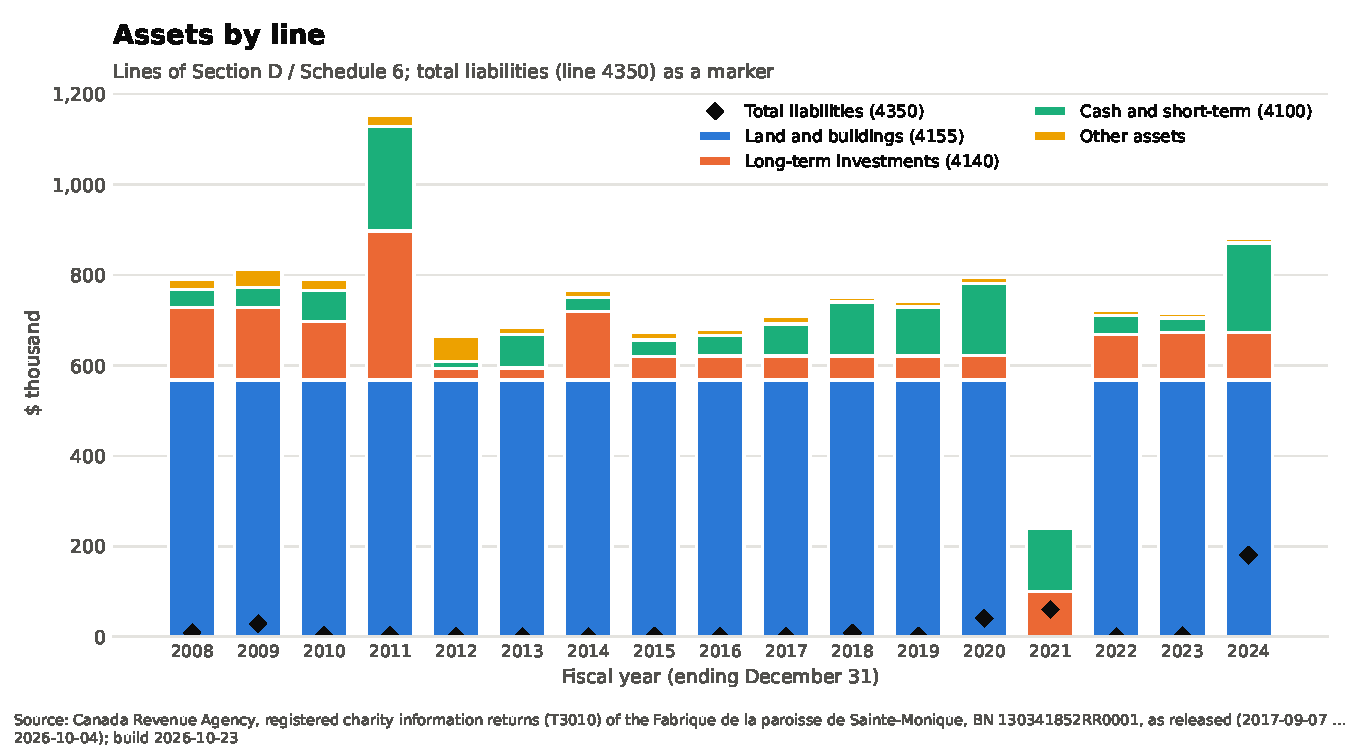
\includegraphics[width=\textwidth]{figures/assets_by_line_en.pdf}\end{center}

Land and buildings are \$567,643 in every year (\$567,642 in 2010 and 2013). Long-term investments (4140) are \$160,000 in 2008--2009, \$130,000 in 2010, \$330,000 in 2011, \$26,124 in 2012, \$26,385 in 2013, \$151,941 in 2014 and \$52,436 to \$53,307 from 2015. Cash and short-term investments (4100) range from \$14,765 (2012) to \$231,051 (2011); they are \$119,181 in 2018. Total liabilities (4350, equal to accounts payable, line 4300, in every year) are \$8 to \$28,711.

\section{What the folder does not contain}

The returns for 2019 and later (to be added as described in section~\ref{sec:prov}); the parish's own financial statements, which its weekly bulletins carried month by month and year by year until 2023 and which are not reproduced here because the bulletins name individuals; any figure for the period after the lane was built in May--June 2024, which will come with the 2024 and 2025 returns once the CRA publishes them.

\section{Reproduction}

\texttt{python3 derived/build.py} rebuilds every table, chart and this note from \texttt{raw/}; \texttt{python3 derived/fetch\_open\_data.py} adds the open-data extracts. The build date and the data's « as of » dates are printed on each chart; this note carries its version in the footer.

\end{document}
